\documentclass[tikz,border=3pt]{standalone}
\usepackage{amsmath}
\usepackage{tikz}
\usepackage{pgfplots}
\pgfplotsset{compat=1.18}
\begin{document}
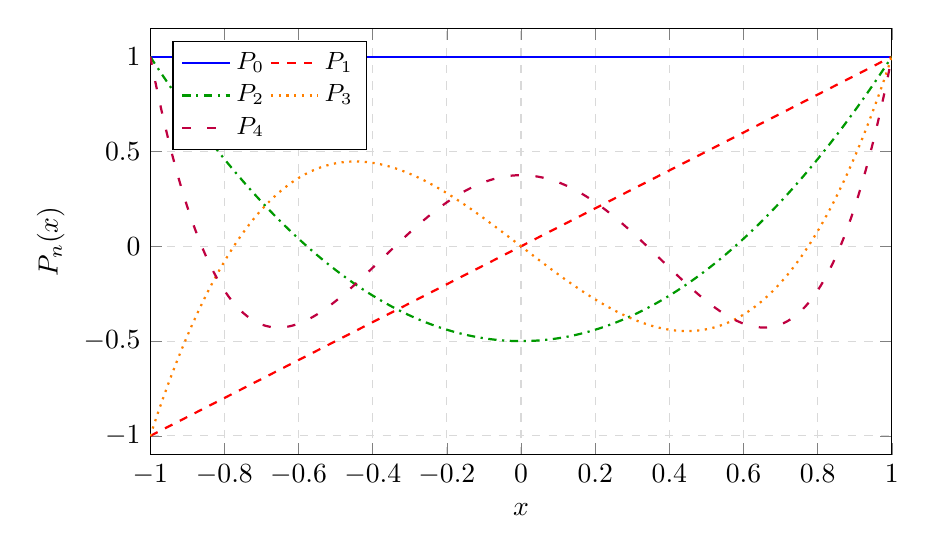
\begin{tikzpicture}
\begin{axis}[
  width=11cm, height=7cm,
  xlabel=$x$, ylabel={$P_n(x)$},
  xmin=-1, xmax=1, ymin=-1.1, ymax=1.15,
  legend style={at={(0.03,0.97)}, anchor=north west, font=\small},
  legend columns=2,
  grid=both, grid style={dashed, gray!30},
  domain=-1:1, samples=200,
  no marks
]
  \addplot[blue, thick, solid]           {1};
  \addlegendentry{$P_0$}
  \addplot[red, thick, dashed]            {x};
  \addlegendentry{$P_1$}
  \addplot[green!60!black, thick, dashdotted] {(3*x^2 - 1)/2};
  \addlegendentry{$P_2$}
  \addplot[orange, thick, dotted]         {(5*x^3 - 3*x)/2};
  \addlegendentry{$P_3$}
  \addplot[purple, thick, loosely dashed]         {(35*x^4 - 30*x^2 + 3)/8};
  \addlegendentry{$P_4$}
\end{axis}
\end{tikzpicture}
\end{document}
